\documentclass{article}

\usepackage{titlesec}
\usepackage{graphicx}
\usepackage{subcaption}
\usepackage{wrapfig}
\usepackage{caption}
\usepackage[
backend=biber,
style=alphabetic,
sorting=ynt
]{biblatex}
\usepackage{tikz, lipsum}
\usetikzlibrary {shapes.callouts}
\usepackage{multicol}

\tikzset{spot/.style={draw, circle, fill=red!20, outer sep=2mm},
    image/.style={outer xsep=3mm, inner sep=1mm, below=6mm, text width=5cm, align=center},
    desc/.style={outer xsep=3mm, inner sep=1mm, text width=5.3cm, align=center}
}

\addbibresource{bibliography.bib} 

\titleformat{\section}[block]{\filcenter\Large\bfseries}{}{1em}{}
\captionsetup[figure]{labelformat=empty}

\title{Roland TR-808: la revolución de las drum machines.}
\author{Ivan Dario Gonzalez Collazos}
\date{Abril 11 del 2023}

\begin{document}

\maketitle

\section{Drum machine: qué es y de donde viene}

La máquina que genera ritmos, patrones y sonidos de percusión a partir de muestras captadas de sonidos de instrumentos reales, o generados a través de circuitos modulando características de una señal para dar como resultado sonidos que simulan los reales\cite{wikidrum}. Esto es llamado el drum machine, un instrumento electrónico musical inventado sobre la década de 1930 pero que empezó a revolucionar la industria musical hacia el final de la decada de 1970.\\

\begingroup
\setlength{\intextsep}{0pt}%
\setlength{\columnsep}{0pt}%

\begin{wrapfigure}{l}{0.48\textwidth}
    \centering
    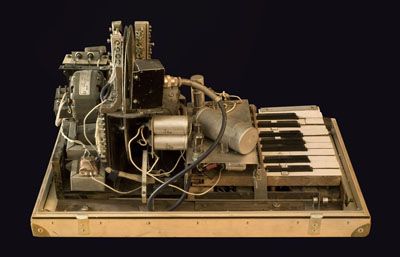
\includegraphics[width=0.38\textwidth]{images/rhythmicon.jpg}
    \vspace{-5pt}
    \caption{Rhythmicon}
\end{wrapfigure}

En la década de 1930 apareceria el primer drum machine: El \emph{Rhythmicon}. Inventado por el ingeniero e inventor ruso Léon Theremin por pedido de Henry Cowell, el cual quería un dispositivo capaz de tocar patrones rítmicos que no se pudiesen tocar en los instrumentos de la época. A pesar de ser bien recibida, solo se vendieron 3 copias.\cite{wikirhythmicon}\cite{drumbook}\\

A finales de la década de 1940, Harry Charmberlin desarrollaría un sistema para leer cintas magnéticas que contenían secuencias rítmicas. Perfeccionando la técnica, en los siguientes años lanzaría el modelo \emph{Model 100 Rhythmate}, vendiendo 10 copias aproximadamente provocando que en las siguientes décadas pudiera lanzar más modelos.\cite{14drums}\cite{drumbook}\\

\endgroup

Hacia el final de la década de 1950, la compañía Wurlitzer lanzaría al mercado el \emph{Side Man}. Este sistema de tubos de vacío y un amplificador de válvulas generan los sonidos, y con un disco rotativo genera los patrones. Además, dejaba seleccionar el tempo, los patrones y botones para tocar cada sonido. Fue popular y construido hasta 1969, siendo usado por artistas de Motown, como Hal Davis.\cite{drumbook}\\

\begingroup
\setlength{\intextsep}{0pt}%
\setlength{\columnsep}{0pt}%

\begin{wrapfigure}{r}{0.45\textwidth}
    \centering
    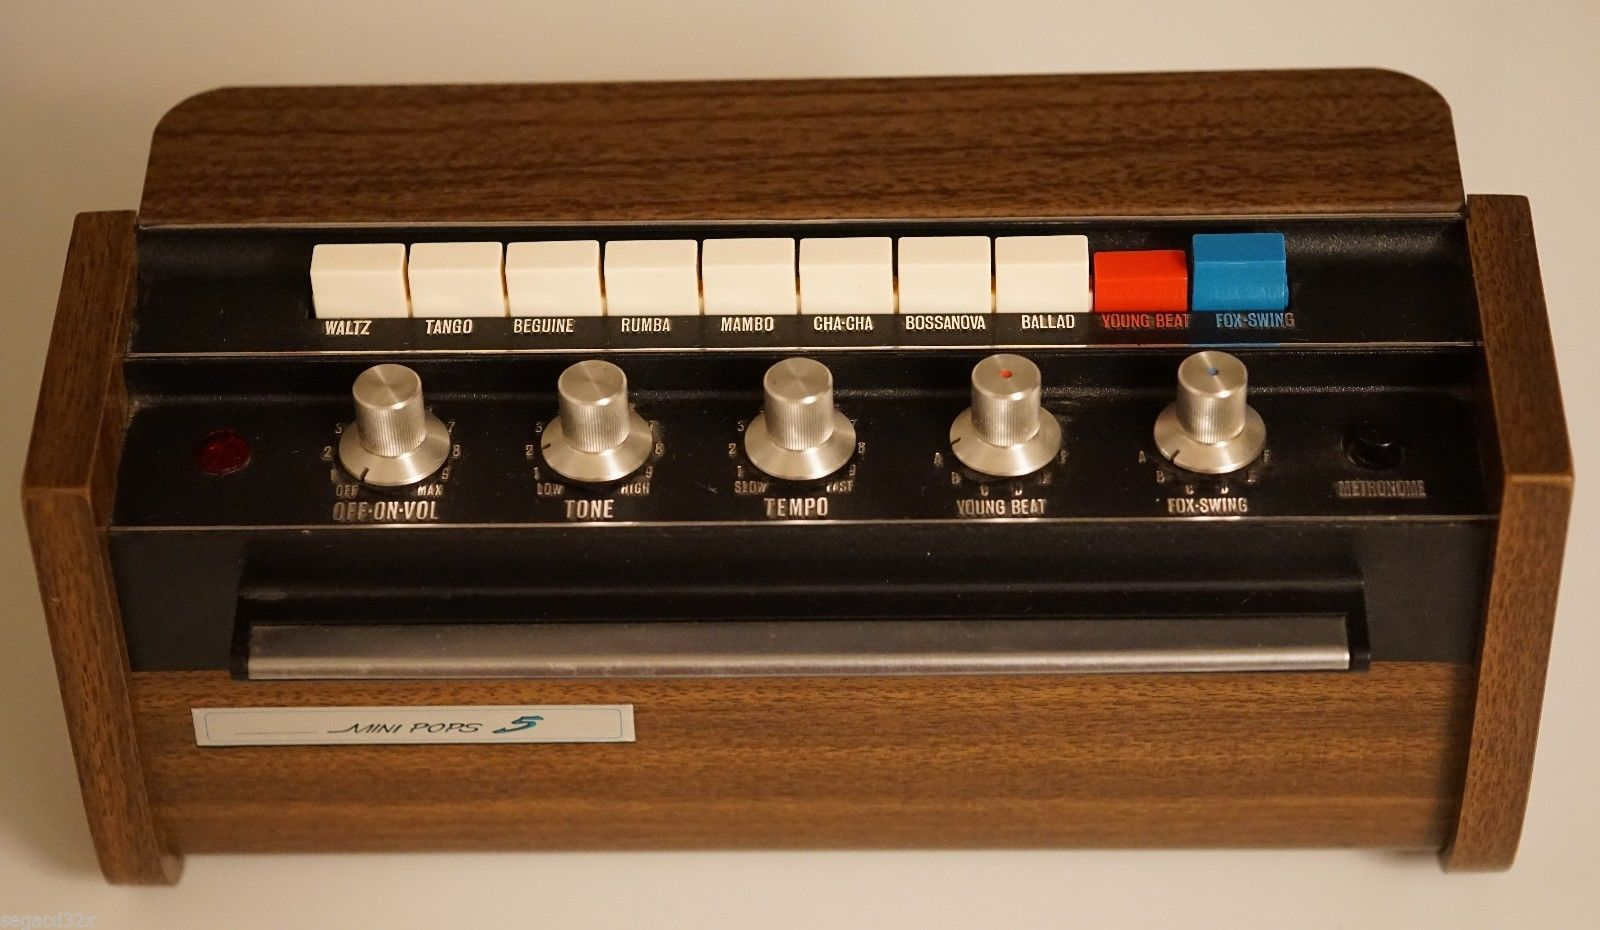
\includegraphics[width=0.35\textwidth]{images/mp5.jpg}
    \vspace{-5pt}
    \caption{Korg MP-5}
\end{wrapfigure}

En 1962, en Japón Tadashi Osanai y Tsutomu Katoh fundarían Keio-Giken (conocida luego como Korg). Estos desarrollarían el \emph{Doncamatic DA-20}, una evolución del Side Man, iterando sobre este modelo presentan el \emph{DC-11} y el \emph{DE-20}; en 1967, Korg lanzaría el Minipops, con sus modelos \emph{MP-5}, \emph{MP-7} y \emph{MP-20}, los cuales son compactos, pero seguían teniendo patrones rítmicos fijos.\cite{drumbook}\\

A mediados de la década de 1970, PAiA Electronics desarrolla el \emph{Programmable Drum Set 3750}, un drum machine programable que permitió a los usuarios guardar sus propios patrones. Utilizada en 1980 por Peter Gabriel, esta fue popular durante un año antes de que las demás compañías desarrollaran sus propios modelos programables.\cite{14drums}\cite{drumbook}\\

\endgroup

\begingroup
\setlength{\intextsep}{0pt}%
\setlength{\columnsep}{0pt}%

\begin{wrapfigure}{l}{0.53\textwidth}
    \centering
    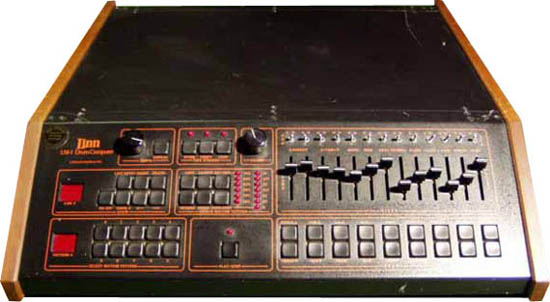
\includegraphics[width=0.43\textwidth]{images/linn.jpg}
    \vspace{-5pt}
    \caption{Linn LM-1}
\end{wrapfigure}

Sobre 1980, Linn Electronics desarrolla su \emph{Linn LM-1}, donde este drum machine grabó los simples de instrumentos físicos dentro de los micro controladores del instrumento, siendo muy popular por su sonido, pero con un precio muy elevado. Artistas como Devo hicieron uso de este drum machine.\cite{14drums}

\endgroup

\section{Roland}

\begingroup
\setlength{\intextsep}{0pt}%
\setlength{\columnsep}{0pt}%

\begin{wrapfigure}{r}{0.5\textwidth}
    \centering
    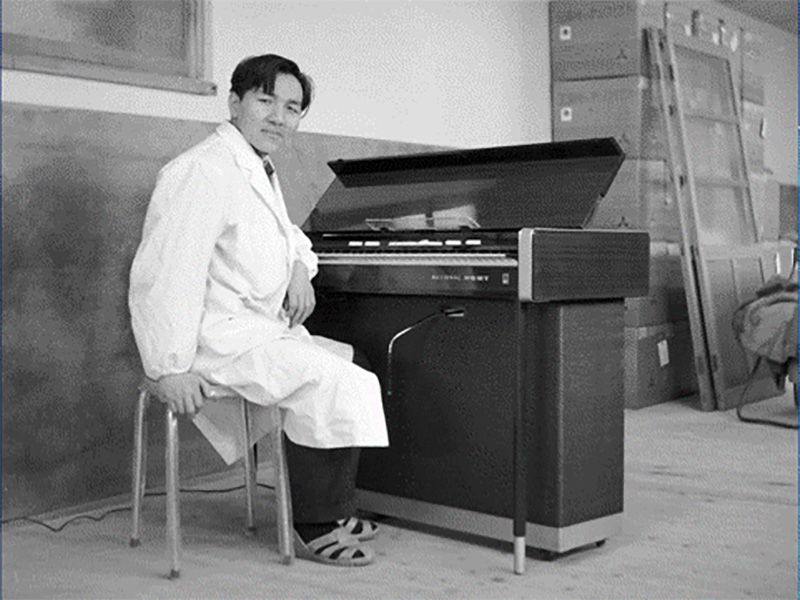
\includegraphics[width=0.4\textwidth]{images/ik.jpg}
    \vspace{-5pt}
    \caption{Ikutaro Kakehashi}
\end{wrapfigure}

Nacido en 1930, Ikutaro Kakehashi creció en Osaka huérfano y durante la segunda guerra mundial trabajo en los talleres de Hitachi donde se desarrollaba diferente armamento para el ejercito japones. Después de la guerra se dedicó a la reparación de relojes y radios donde fundaría diferentes pequeños negocios que lo ayudarían para tratar de pagar estudios formales en Osaka.\cite{rolandstory}\\

Cuando llega a Osaka, casi muere a causa de tuberculosis y pasa varios años en el hospital batallando la enfermedad hasta que un tratamiento experimental lo cura; en medio de estos años se sostiene arreglando relojes y radios a pacientes y trabajadores del hospital.\cite{rolandstory}\\

\endgroup

Cuanto sale del hospital, decide fundar una tienda de reparación de radios, que con los años se transformaría en Ace Electrical Company. En 1955 decide expandir sus intereses hacia la creación de instrumentos que pudieran producir melodías, experimentando desde ese año hasta 1960, donde lanza el órgano \emph{Technics SX601}, que pondría a Ace en el mapa de las compañías de equipo musical.\cite{rolandstory}\\

\begingroup
\setlength{\intextsep}{0pt}%
\setlength{\columnsep}{0pt}%

\begin{wrapfigure}{r}{0.5\textwidth}
    \centering
    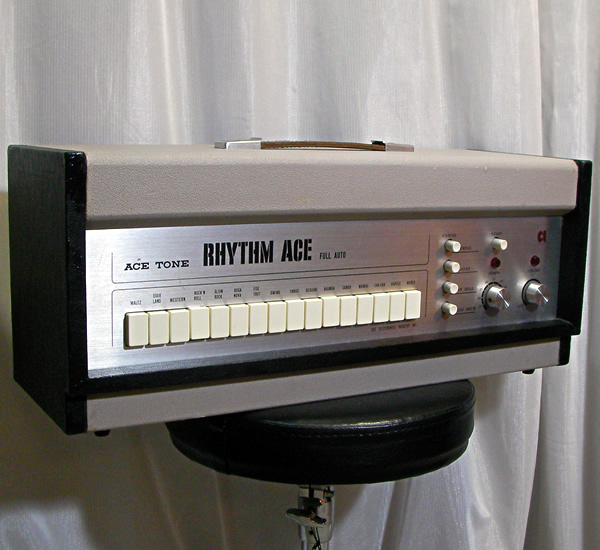
\includegraphics[width=0.4\textwidth]{images/fr1.jpg}
    \vspace{-5pt}
    \caption{FR1 Rhythm Ace}
\end{wrapfigure}

En 1964, Ace lanza el \emph{R1 Rhythm Ace}, un fracaso debido a que no tenía patrones pre programados. Pero Kakehashi junto con sus colegas desarrollarían la “matriz de diodos”, que permitiría dicha función y con esto nacería el \emph{FR1 Rhythm Ace} en 1967, que con su popularidad permitió la alianza con Hammond Internacional. Con esta alianza, Ace alcanzaría una facturación de 40 millones de dólares por año, pero sería comprada por Sumitomo Chemical, cambiando la visión que tenía Kakehashi sobre el negocio, lo que llevaría a que dejara la empresa en 1972.\cite{rolandstory}\cite{drumbook}\\

\endgroup

\begingroup
\setlength{\intextsep}{0pt}%
\setlength{\columnsep}{0pt}%

\begin{wrapfigure}{l}{0.5\textwidth}
    \centering
    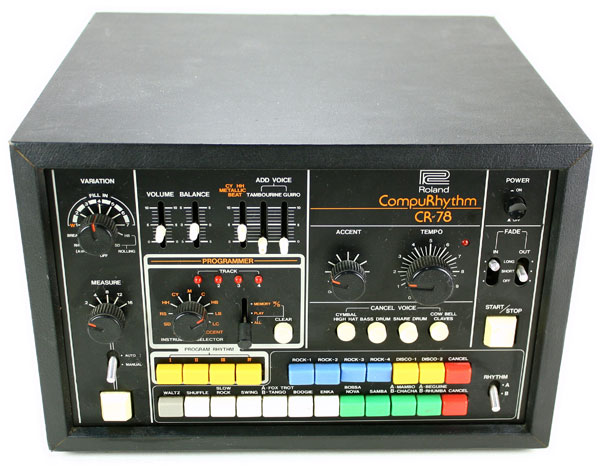
\includegraphics[width=0.4\textwidth]{images/cr78.jpg}
    \vspace{-5pt}
    \caption{Roland CR-78}
\end{wrapfigure}

Kakehashi fundaría Roland tan solo un mes después de salir de Ace, con un capital US \$ 100.000, un puñado de empleados y sin productos. Entonces, apelan al mercado internacional y haciendo una gira de negocios por USA, Canadá y Europa obtiene presupuesto para empezar la producción de los modelos \emph{TR-33}, \emph{TR-55} y \emph{TR-77}.\cite{rolandstory}\\

En 1978, Roland lanza el \emph{CR-78}, una de las primeras drum machine en llevar microprocesador, haciendo uso del switch de escritura WS-1 donde la combinación entre la programación y los ritmos pregrabados hizo que fuera muy popular y fuera usada por artistas como Blondie o Phil Collins.\cite{14drums}

\endgroup

\section{TR-808: La revolución}

En 1980, un lote de transistores defectuosos lleva a Roland a construir durante tres años el drum machine que cambio el curso de la música para siempre.\cite{808film}\\

\emph{TR-808}, fue el modelo producido por Roland durante entre los años de 1980 y 1983, vendido por un precio de US \$ 1.195 dólares fue criticado por su sonido poco natural y muy inferior según la crítica especializada a la contemporánea, pero mucho más costosa Linn LM-1.\\

\begingroup
\setlength{\intextsep}{0pt}%
\setlength{\columnsep}{0pt}%

El 808 se caracteriza por un sonido particular, donde sus diferentes componentes no suenan como los instrumentos reales y según muchos productores, como Rick Rubin por ejemplo, tiene un sonido único que no se asemeja a otra drum machine del mercado a inicios de la década de 1980.\\

\begin{wrapfigure}{r}{0.4\textwidth}
    \centering
    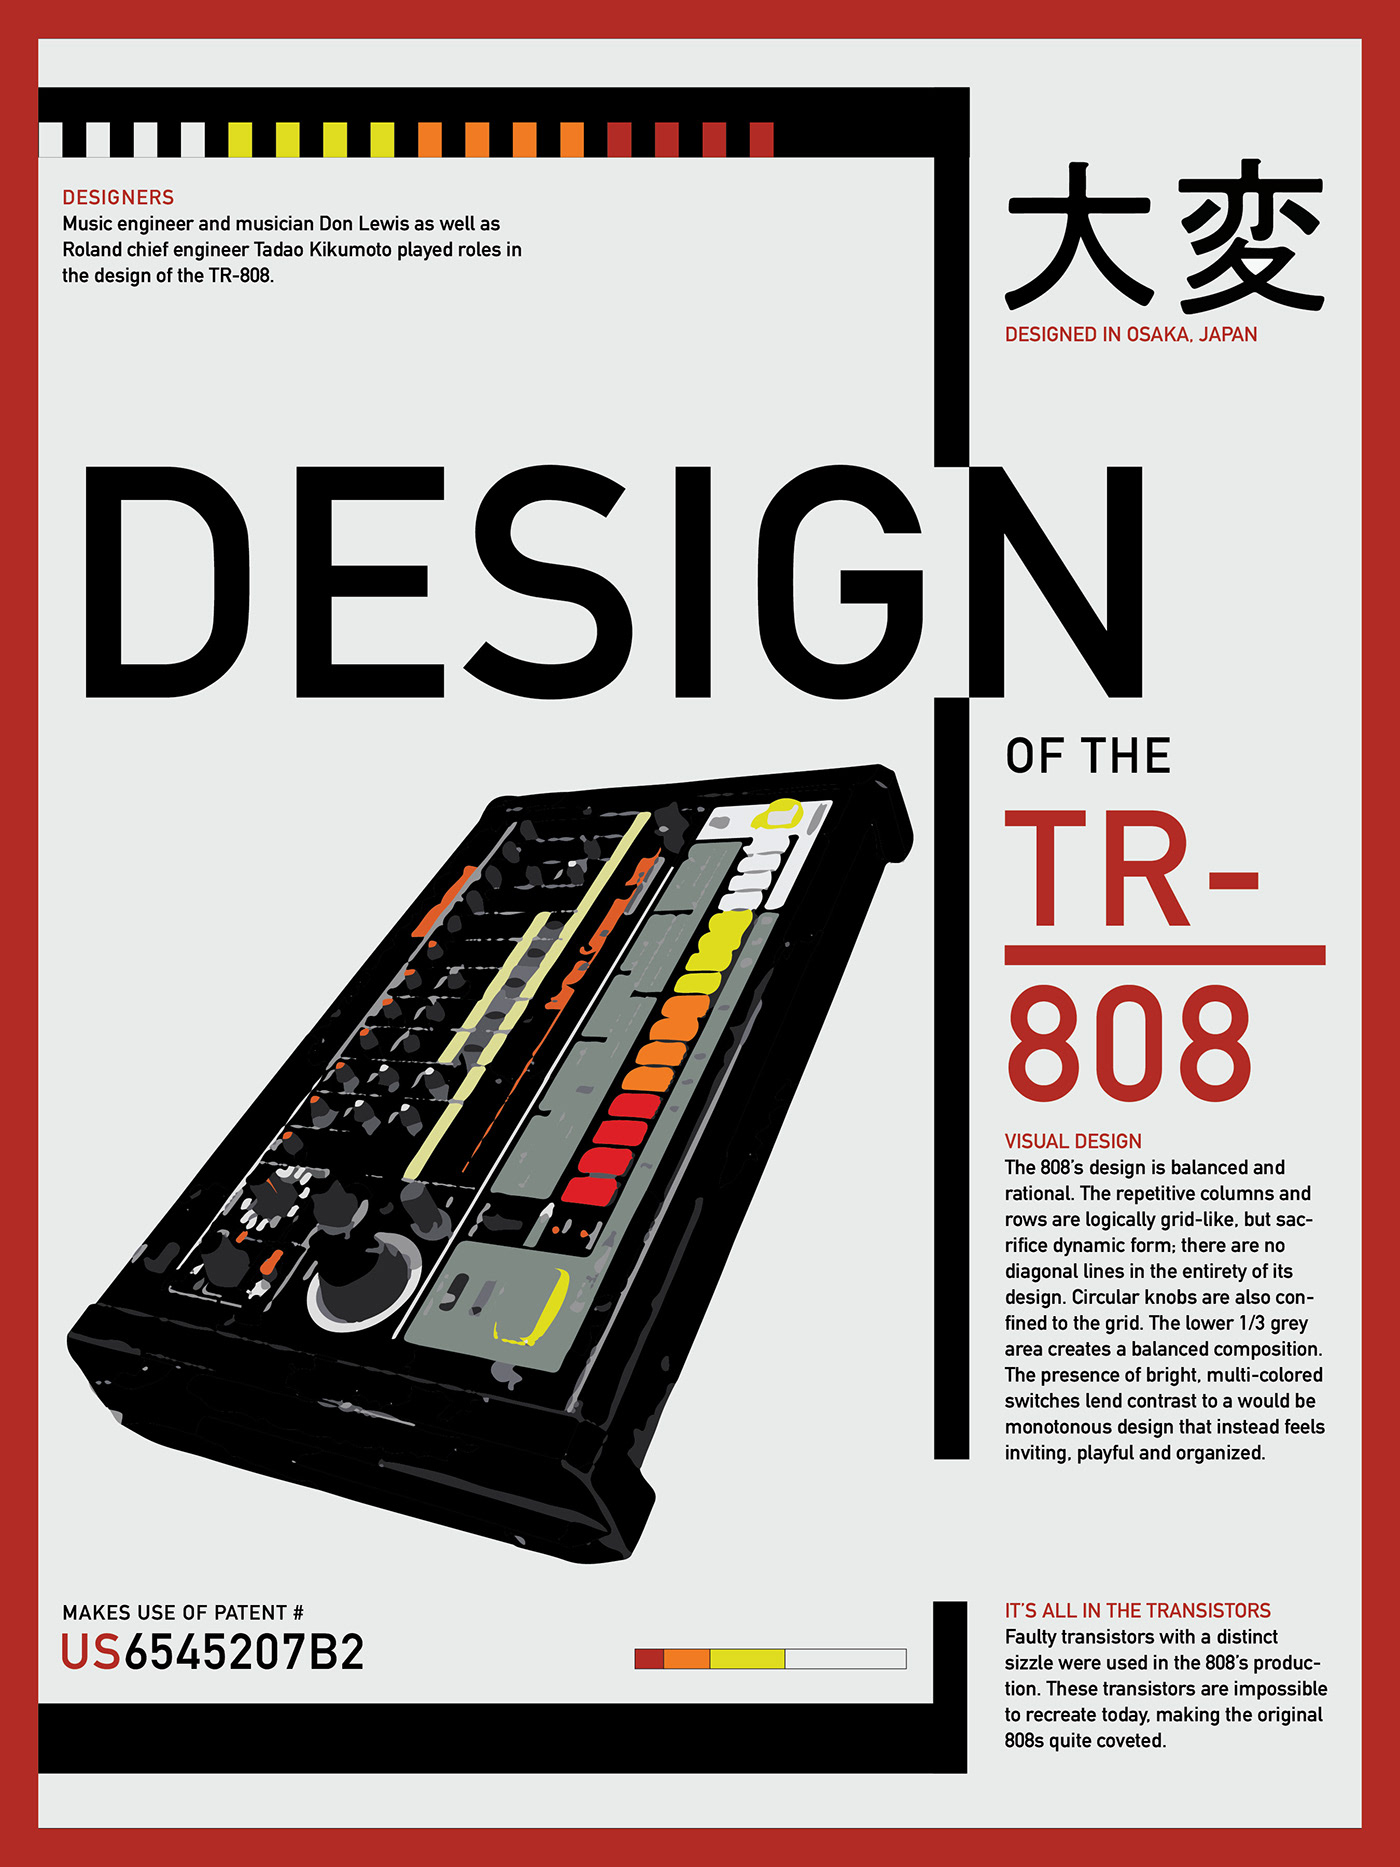
\includegraphics[width=0.3\textwidth]{images/808ad.jpg}
    \vspace{-5pt}
    \caption{Roland TR-808 AD}
\end{wrapfigure}

Los sonidos que puede generar la 808 son\cite{808tspecs}:

\begin{multicols}{3}
    \begin{itemize}
        \item Bass Drum
        \item Snare Drum
        \item Low Conga
        \item Low Tom Tom
        \item Mid Conga
        \item Mid Tom Tom
        \item Hi Conga
        \item Hi Tom Tom
        \item Claves
        \item Rim Shot
        \item Maracas
        \item Hand Clap
        \item Cow Bell
        \item Cymbal
        \item Open Hi Hat
        \item Closed Hi Hat
    \end{itemize}
\end{multicols}

\endgroup

\begingroup
\setlength{\intextsep}{0pt}%
\setlength{\columnsep}{0pt}%

\begin{wrapfigure}{l}{0.6\textwidth}
    \centering
    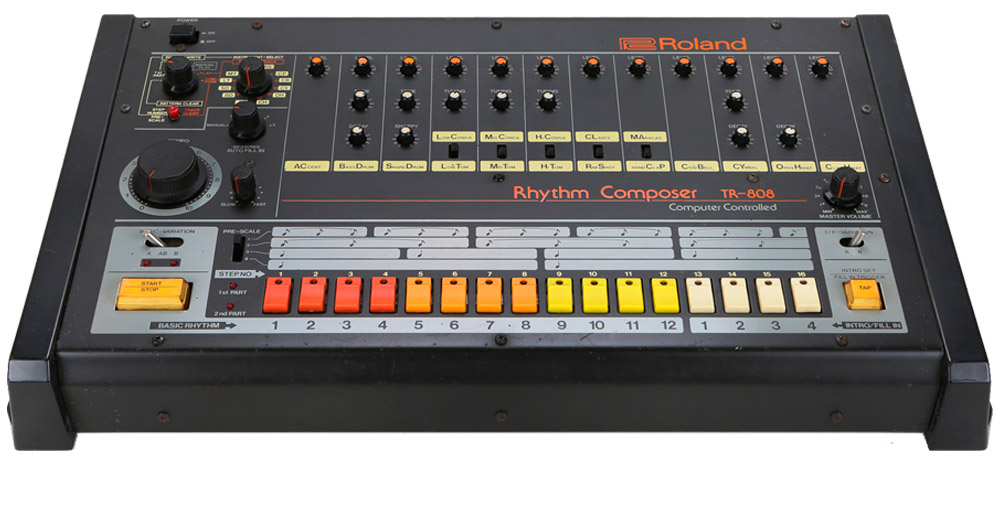
\includegraphics[width=0.5\textwidth]{images/tr808.jpg}
    \vspace{-3pt}
    \caption{Roland TR-808}
\end{wrapfigure}

Uno de los sonidos mas peculiares y utilizados del 808 es su Bass Drum, ya que este kick da un muy buen registro de bajo y muchos productores sacaran provecho de este sonido generando bass drums muy profundos, con mucho cuerpo y un ataque que no se podia encontrar en otros instrumentos electrónicos de la época. Este fenómeno se dio en Miami, una de las ciudades donde la 808 cambio el panorama musical.\cite{808film}\\

Además de su sonido único, el TR-808 se caracteriza por programar hasta 32 patrones rítmicos, con acentuaciones, en diferentes tempos y en diferentes medidas de tiempo, que además de contar con un 4/4 incluye medidas de tiempo como 5/4 y 7/8. También incluye volumen para cada uno de los sonidos y salidas para sincronizar con sintetizadores que utilizaran DIN Sync\cite{wiki808}.

\endgroup

\section{El legado de la 808}

El impacto de la de la 808 empieza a verse en Japón, donde la banda Yellow Magic Orchestra empezó a utilizarlo tanto en sus presentaciones en vivo como en sus álbumes.\\

\begingroup
\setlength{\intextsep}{0pt}%
\setlength{\columnsep}{0pt}%

\begin{wrapfigure}{r}{0.45\textwidth}
    \centering
    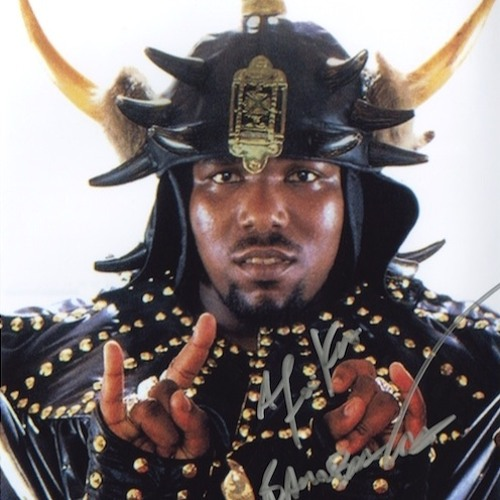
\includegraphics[width=0.35\textwidth]{images/afrika.jpg}
    \vspace{-5pt}
    \caption{Afrika Bambaataa}
\end{wrapfigure}

Pero fue en New York donde \emph{Afrika Bambaataa}, un DJ de la escena Hip-Hop utiliza en su primera producción el 808 influenciado por los japoneses, donde Planet Rock en 1982 fue el Genesis de lo que hoy conocemos como Hip-Hop.\cite{808film}\\

Aun en 1982 y buscando quitarse la influencia de Motown, \emph{Marvin Gaye} se traslada a Bélgica donde en busca de nuevos sonidos e independencia para sus composiciones, empieza a grabar su álbum Midnight Love que contiene uno de sus éxitos más grandes, Sexual Healing, provocando que en el pop y RnB se empezara a utilizar la 808 en grandes producciones de grandes artistas.\cite{808film}\cite{slaves}\\

\endgroup

\begin{figure}[h]
    \begin{center}
        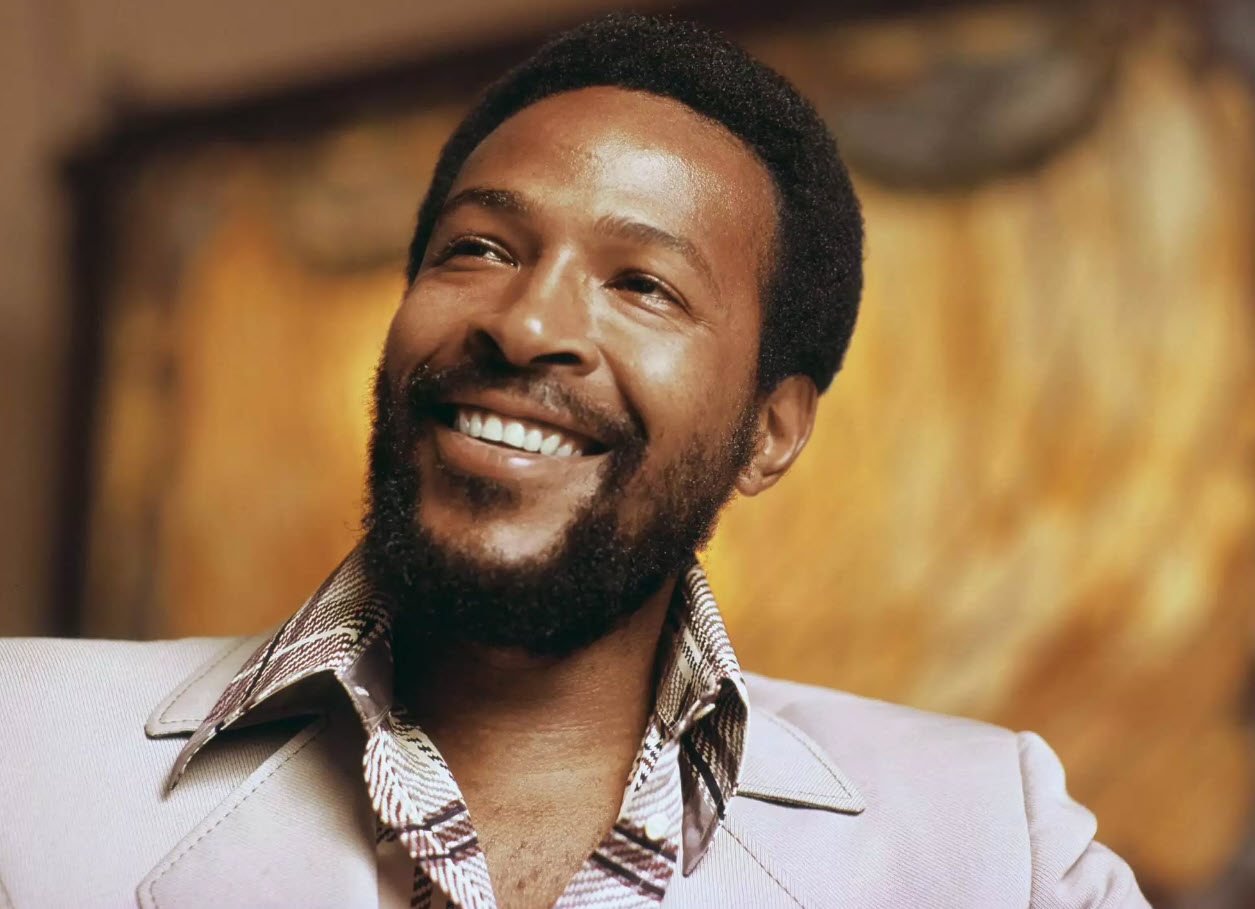
\includegraphics[scale=0.2]{images/marvin.jpg}
    \end{center}
    \vspace{-5pt}
    \caption{Marvin Gaye}
\end{figure}

\begingroup
\setlength{\intextsep}{0pt}%
\setlength{\columnsep}{0pt}%

\begin{wrapfigure}{r}{0.5\textwidth}
    \centering
    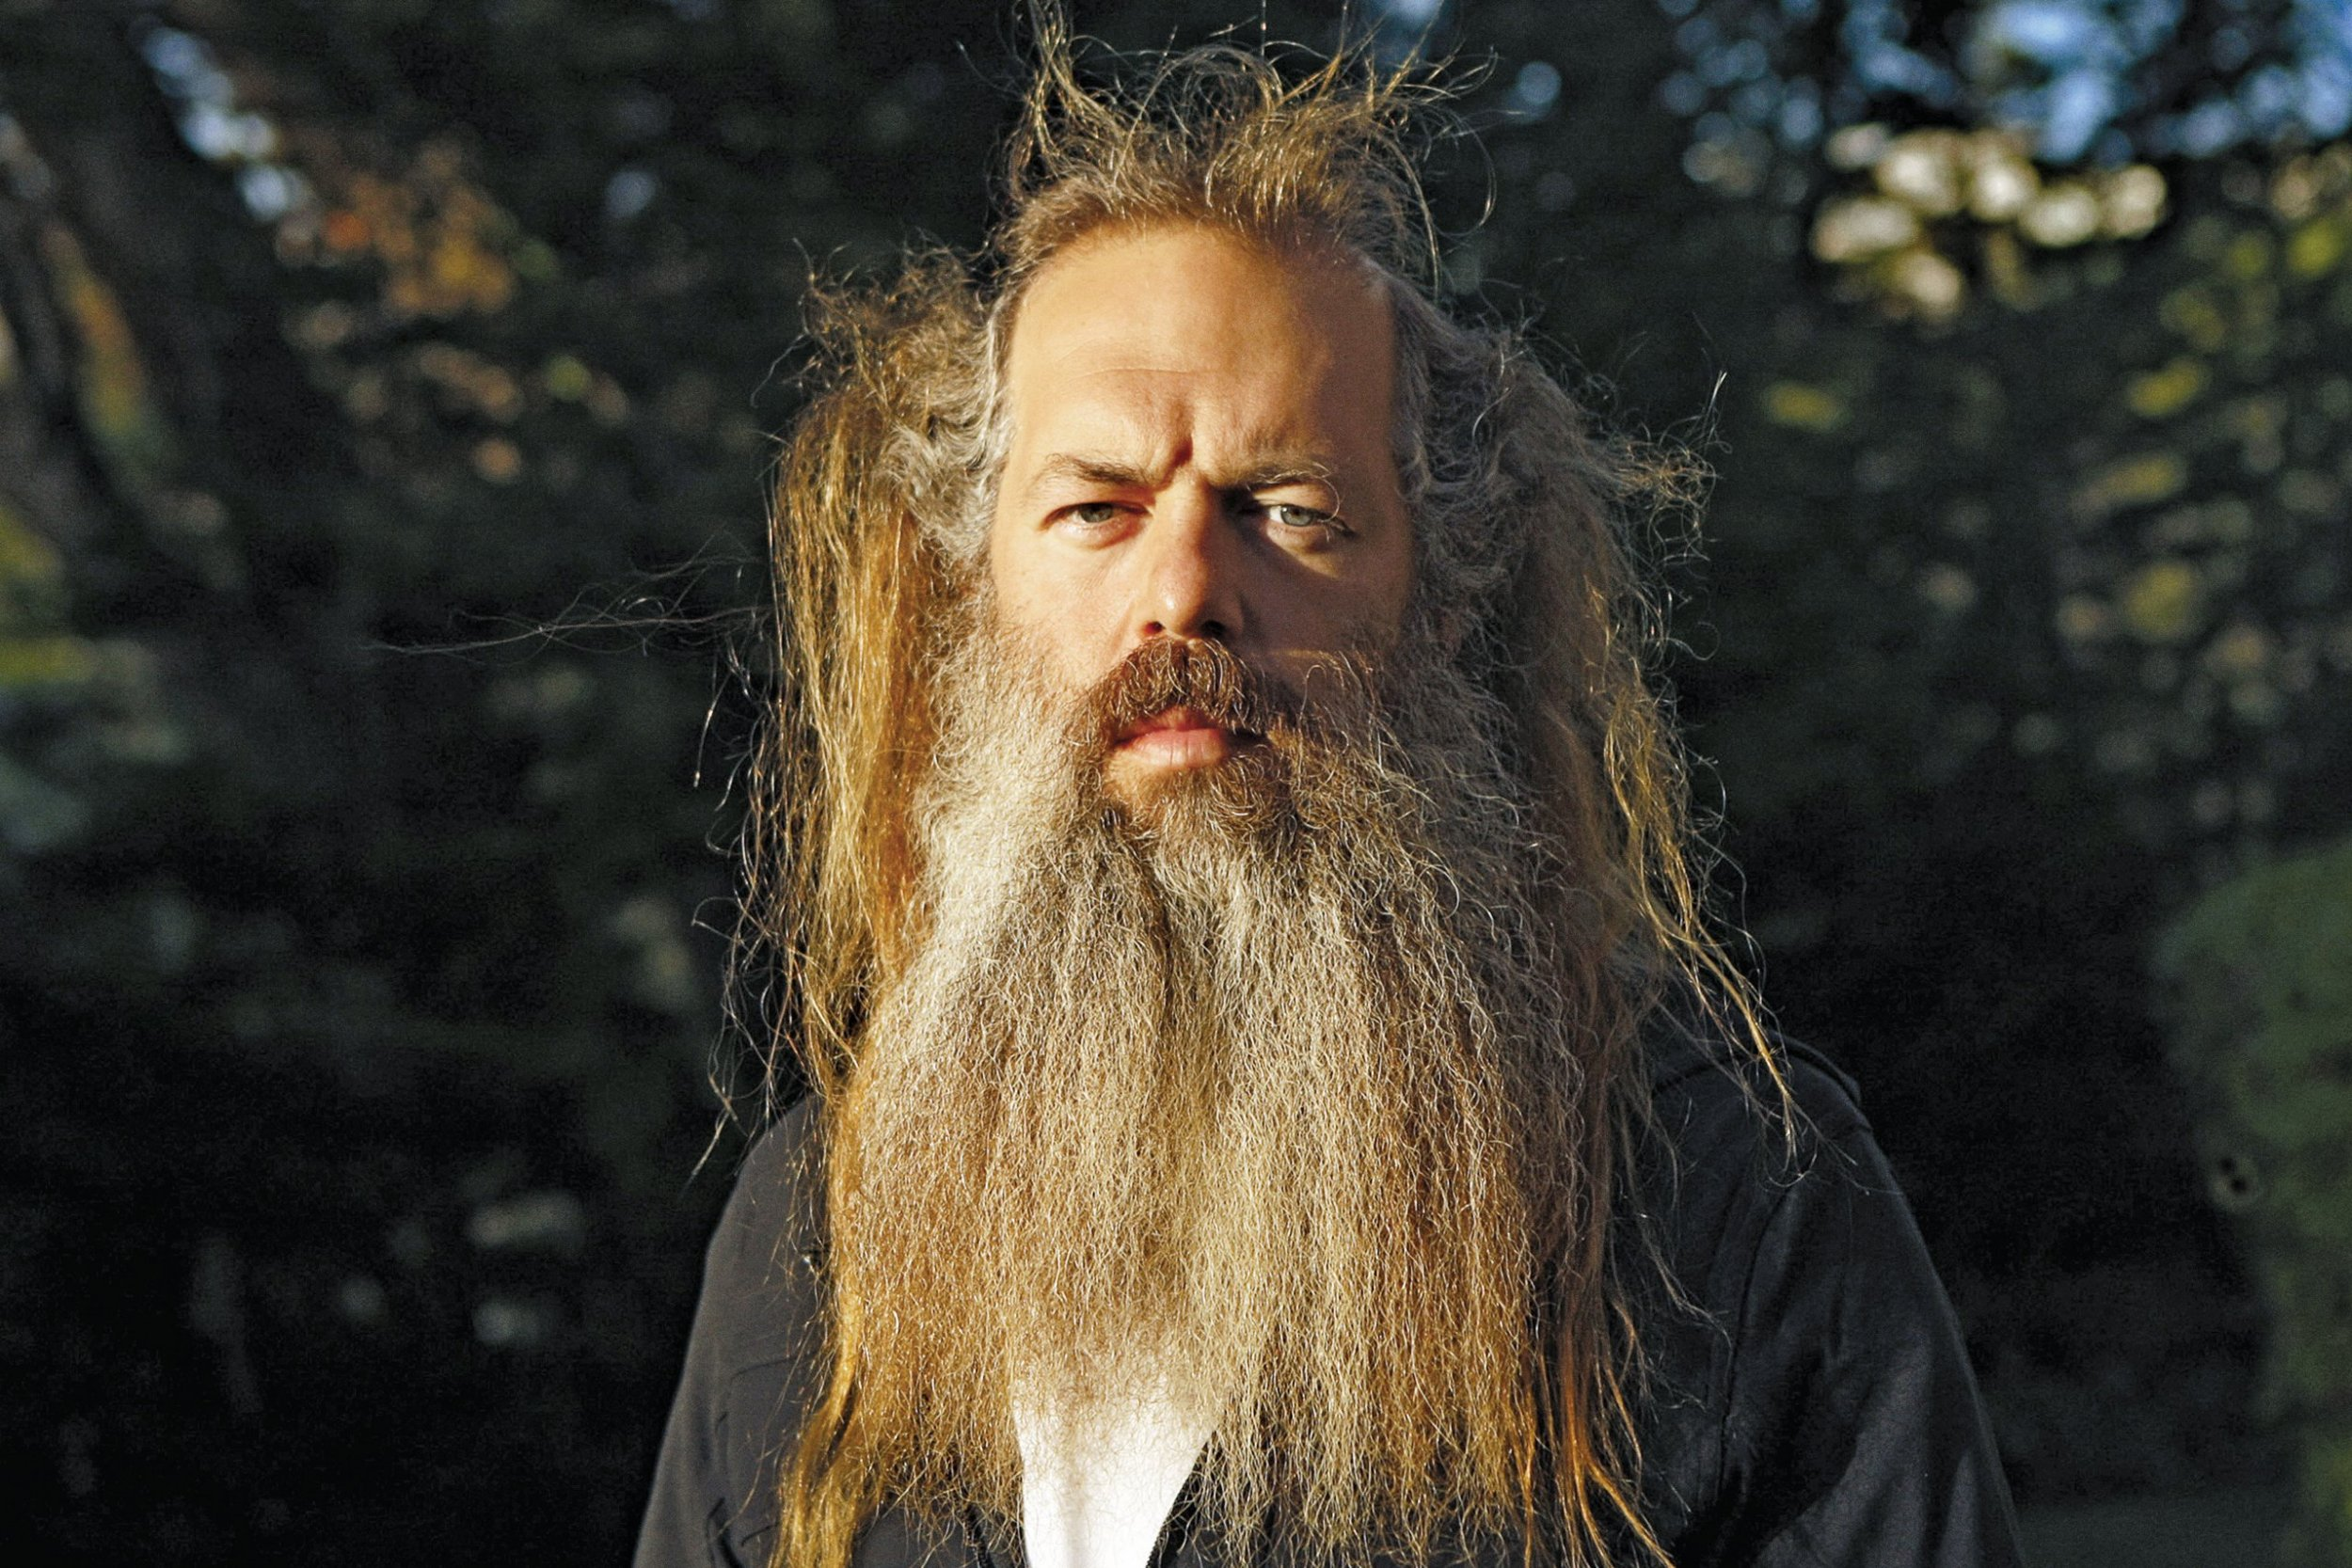
\includegraphics[width=0.4\textwidth]{images/rubin.jpg}
    \vspace{-5pt}
    \caption{Rick Rubin}
\end{wrapfigure}

Unos años después, \emph{Rick Rubin} empezaría producir diferente MCs de New York que incluirían beats creados en la 808, siendo uno de los resultados más conocidos los Beastie Boys, con su álbum \emph{Licence to Ill} y con el track más representativo de la 808 en ese álbum: Paul Revere.\cite{808film}\\

Pronto, la escena del Hip-Hop se popularizo con nombres como LL Cool J y Public Enemy produciendo los beats de sus canciones en 808s.\cite{808film}\\

\endgroup

\begingroup
\setlength{\intextsep}{0pt}%
\setlength{\columnsep}{0pt}%

\begin{wrapfigure}{l}{0.5\textwidth}
    \centering
    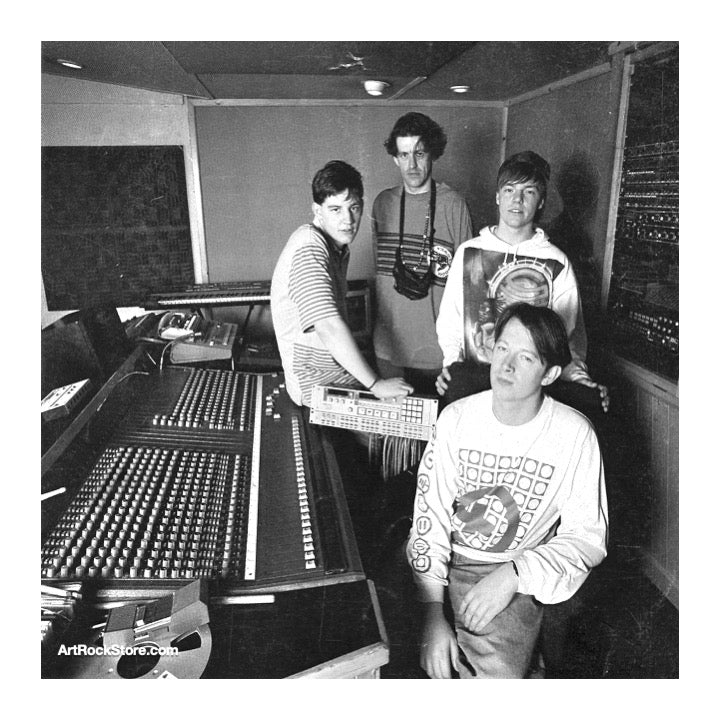
\includegraphics[width=0.4\textwidth]{images/808state.jpg}
    \vspace{-5pt}
    \caption{808 State}
\end{wrapfigure}

Pero no todo fue pop e hip-hop, la 808 ayuda a cimentar la base de la música electrónica empezando por el House y sus variantes, en ciudades como Chicago y Detroit en USA; en estas cuidades se originarían las primeras canciones de \emph{Acid House y Drum and Bass}, que ayudarían popularizar el género en las discotecas underground de la época.\cite{808film}\\

Pero su influencia no paro allí, ya que aun en el siglo 21 artistas como Usher, Kanye West y Jay Z han utilizado beats construidos en 808, con Kanye haciendo un álbum tributo y a su vez componiendo los beats en un Roland TR-808.\cite{808film}\\

\endgroup

Aquí un breve resumen de los álbumes y canciones que fueron populares haciendo uso de la legendaria Roland TR-808:\\

\begin{tikzpicture}
    \draw[thick](0,7)
        --(0,7)node[spot](a1){}
            node[image, left]{
                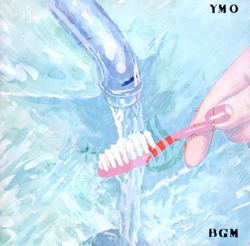
\includegraphics[width=0.7\textwidth]{images/ymo.jpg}
            }
            node[desc=a1.east, right]{Yellow Magic Orchestra}
        --(0,3)node[spot](a1){}
            node[image, right]{
                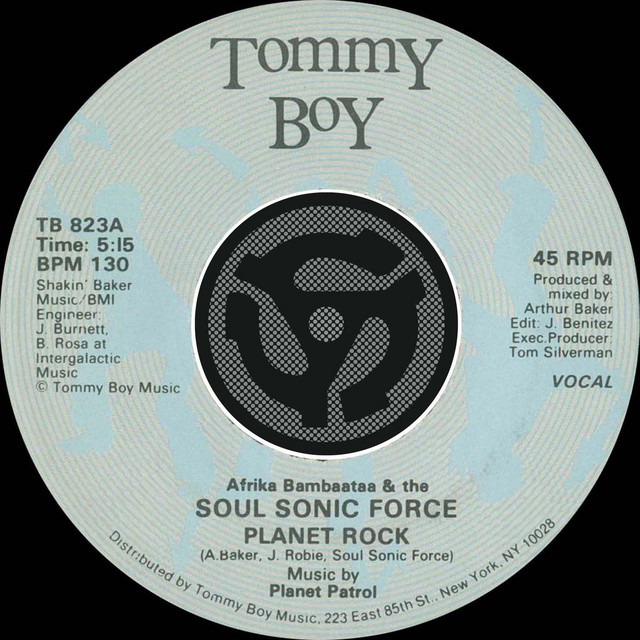
\includegraphics[width=0.7\textwidth]{images/planet.jpg}
            }
            node[desc=a1.west, left]{Afrika Bambaataa \& The Soulsonic Force}

        --(0,0);
    \end{tikzpicture}
    
    \begin{tikzpicture}
        \draw[thick](0,19)
            --(0,18)node[spot](a1){}
                node[image, left]{
                    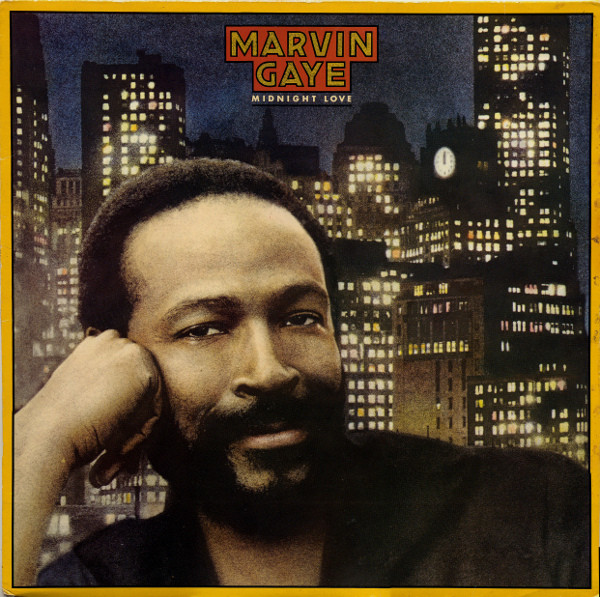
\includegraphics[width=0.7\textwidth]{images/marvin808.jpg}
                }
                node[desc=a1.east, right]{Marvin Gate}
            --(0,14)node[spot](a1){}
                node[image, right]{
                    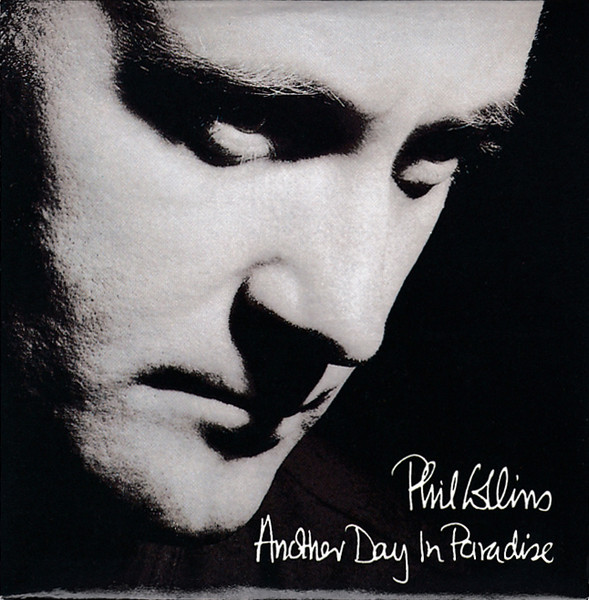
\includegraphics[width=0.7\textwidth]{images/phil.jpg}
                }
                node[desc=a1.west, left]{Phil Collins}
            --(0,10)node[spot](a1){}
                node[image, left]{
                    
\includegraphics[width=0.7\textwidth]{images/public.jpg}
                }
                node[desc=a1.east, right]{Public Enemy}
            --(0,6)node[spot](a1){}
                node[image, right]{
                    
\includegraphics[width=0.7\textwidth]{images/808album.png}
                }
                node[desc=a1.west, left]{808 State}
            --(0,2)node[spot](a1){}
                node[image, left]{
                    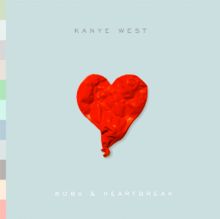
\includegraphics[width=0.7\textwidth]{images/808kanye.png}
                }
                node[desc=a1.east, right]{Kanye West}
            --(0,0);
        \end{tikzpicture}

\nocite{*}

\printbibliography[
title={Bibliografía}
]

\end{document}